\subsection{The cell}
\label{sec:cell}
Cells are the fundamental units of every living being, which can be made up of one cell (unicellular) or more (multicellular).
Independently on how big and complex an organism could be, each cell always maintains its individuality and its independence but maintaining common structural proprieties.

We distinguish between prokaryotic and eukaryotic cells. 
The first ones are typically unicellular organisms and don't encapsulate the genetic material (\gls{dna}) inside the nucleus.
While the second ones protect the genetic material inside a specific organelle called nucleus, protected by membranes.

For any kind of cell, the internal volume is defined by the \textit{cytoplasm}, which is a liquid solution where several insoluble particles stand, such as enzymes, \textit{RNA} and metabolites.

Moreover, it is possible to distinguish multiple organelles, such as \textit{ribosomes}, the \textit{endoplasmic reticulum}, the \textit{golgi comples},\textit{lisosomes} and the, for euokaryotic cells, \textit{nucleus} (figure \ref{fig:cell}).

\begin{figure}[h]
\centering
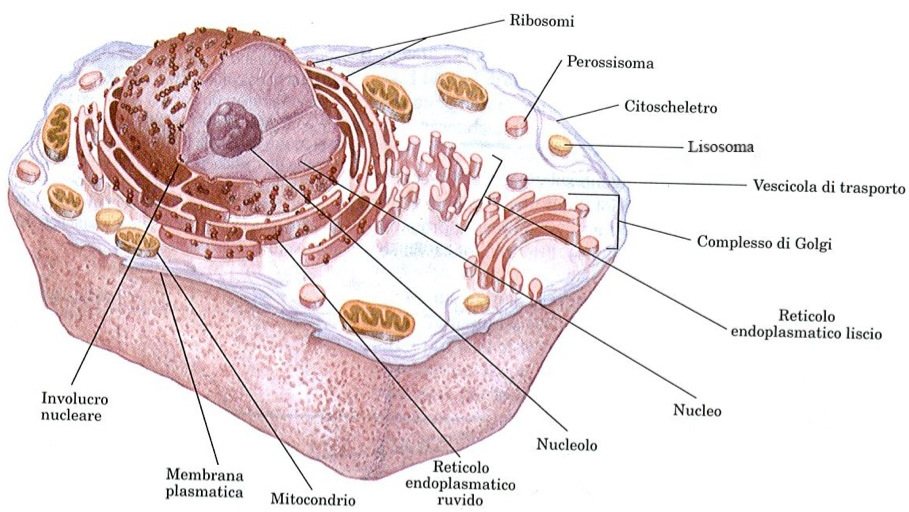
\includegraphics[width=10cm, keepaspectratio]{img/intro/cell.png}
\caption[The Cell]{Schematic representation of an Eukaryotic Cell.}
\label{fig:cell}
\end{figure}

\subsection{The DNA}
\label{sec:genica}
The \textit{DNA} was been isolated for the first time by the German doctor Friedrich Miescher in 1869, while in the same decade the English biologist Charles Darwin was publishing \textit{On the Origin of the Species} and the  Augustinian friar scientist was communicating his results on the pees to the Brunn Natural History Society.

Because the substance isolated by Miescher was white, lightly acid and present only into the cells nuclei, it was been termed \textit{Nucleic Acid}.
Name modified afterwards in \gls{dna}, to distinguish is from another one, very similar, the \gls{rna}.

These two molecules are constituted by \textit{nucleotides}, constituted by a nitrogen base, deoxyribose sugar and a phosphate group.
We distinguish two nitrogen bases, purines and pyrimidines.
Inside the \gls{dna}, we have two \textit{pyrimidines}, \textit{adenine (A)} and \textit{guanine (G)}, and two \textit{pyrimidines}, the \textit{Cytosine (C)} and the \textit{Thimine (T)}  .
Inside \gls{rna} \textit{Thymine} is substituted by the \textit{Uracil (U)}.

\begin{figure}[h]
\centering
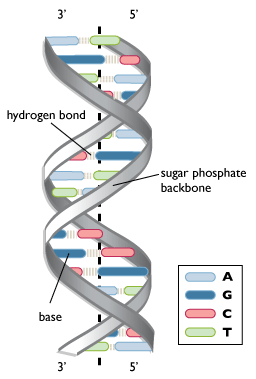
\includegraphics[width=5cm, keepaspectratio]{img/intro/dna1.png}
\caption[the \gls{dna}]{Schematic representation of double-stranded filament structure of \gls{dna}. The legend report the four nitrogen bases, Adenine, Guanine, Cytosine and Thymine.}
\label{fig:dna}
\end{figure}

\gls{dna} structure (figure \ref{fig:dna}) was discovered, in the '50s, by the American scientist James Watson, the French physicist Francis Crick and the English chemist-physicist Rosalind Franklyn.
According to their model, the \gls{dna} is a double-stranded filament, where Adenines can pair only with Thymines and Guanines only with Cytosines.
The four bases constitute the alphabet for the genetic message.

\gls{dna} is folded on itself (\textit{\gls{dna} packaging}, thanks to specific "beads" called \textit{nucleosomes}, which themselves consist of eight proteins with tails, called \textit{histones}, that have the \gls{dna} wrapped on them.
This mechanism enables to store around 2 meters of chromatin inside a nucleus of a 2-10 micron diameter when referring to Human species.

\begin{figure}[h]
\centering
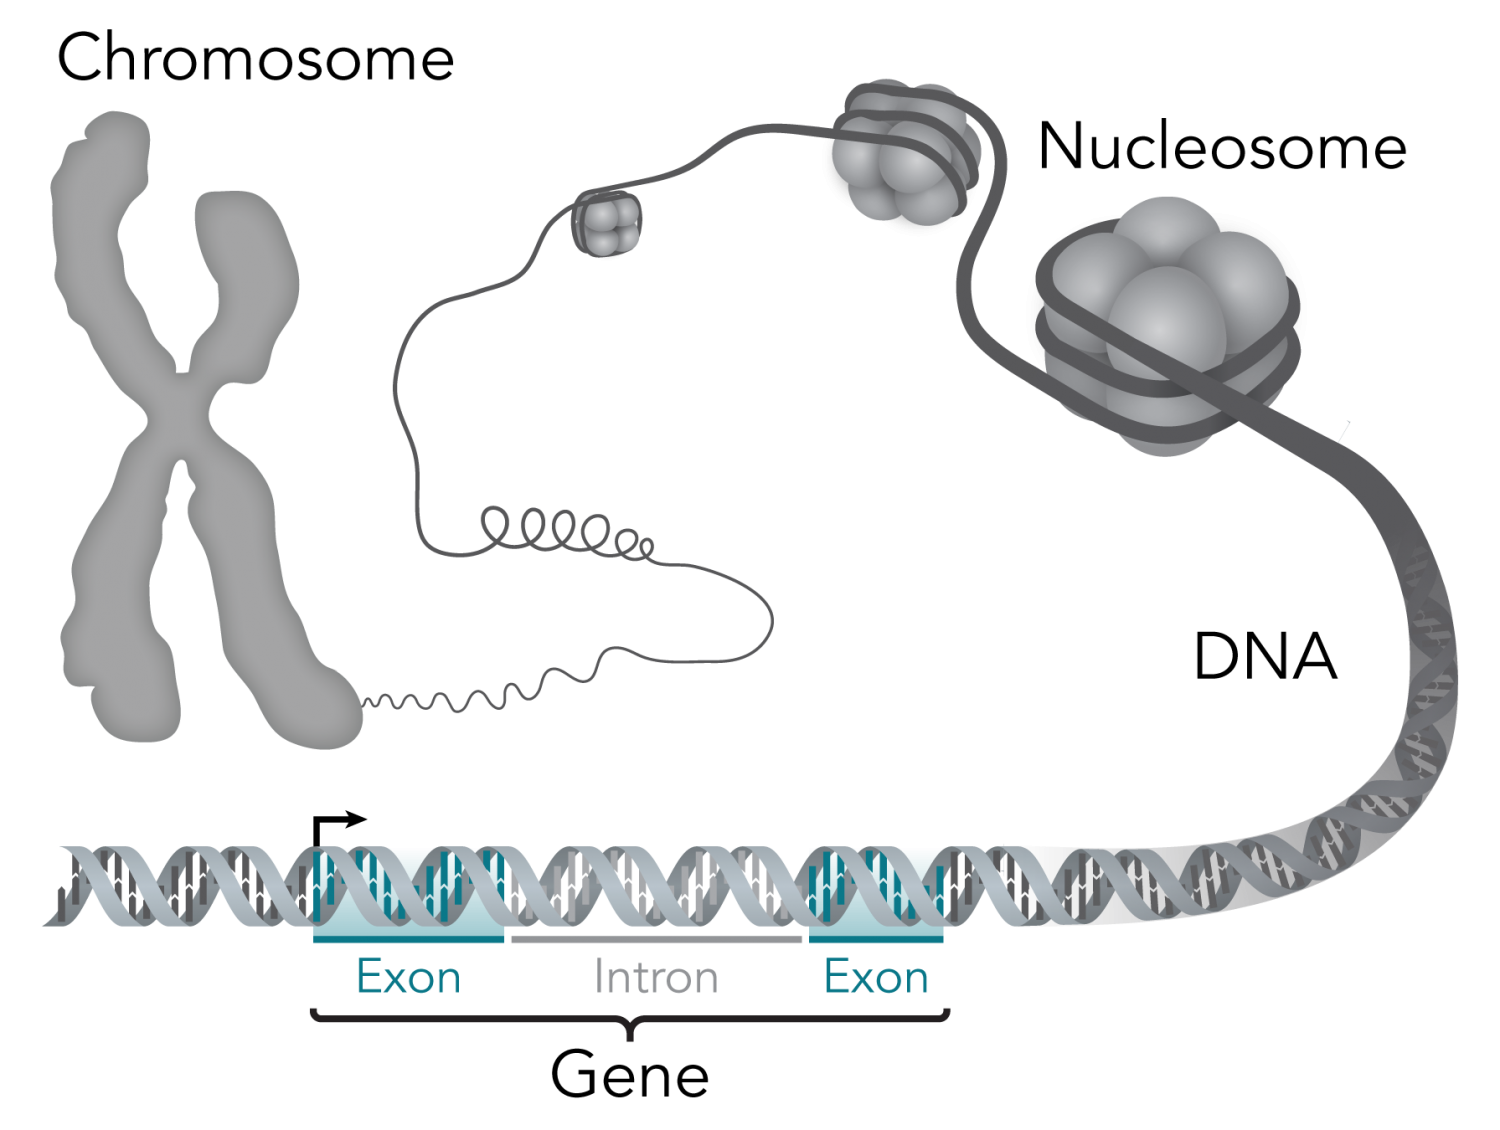
\includegraphics[width=8cm, keepaspectratio]{img/intro/gene_chrom.png}
\caption[Gene Chromosome relation]{Representation of the relation between the chromosome and the gene. 
A gene stands on a portion of a chromosome, which is rolled around a nucleosome.
Each gene is composed by introns and exons. When transcripted, the first ones are involved in post-transcriptional cellular mechanisms, while the second ones are destined to be translated into proteins.}
\label{fig:dnachromgene}
\end{figure}

Moreover, the \gls{dna} contains the \textit{genes}, particular sections containing relevant information for building proteins and other fundamental molecules for the cellular behaviour regulation.
Each gene is localized on a precise position of a \textit{Chromosome}, which are in a different number for each species.
Each chromosome is constituted by \gls{dna} within thousands of genes, each one composed by introns and exons (figure \ref{fig:dnachromgene}).

It is important to underlying that since some decades ago the \textit{Central Dogma of Molecular Biology} was founded on the transcription-translation principle, where \textit{exons} were transcribed into \gls{rna}, which subsequently it would have been translated into protein.

Nowadays, we know that the gene transcription is regulated by several mechanisms, and moreover, the translation is not the only process fated for \gls{rna}.

Indeed, since few years ago, introns were considered junk \gls{dna}, but now demonstrated to be involved in regulation mechanisms, such as post-transcriptional processes, while exons are destined to be translated into proteins (figure \ref{fig:dnachromgene}).


\subsection{The Chromatin}
\label{sec:chromatin}
In order to fit inside the eukaryotic cells nucleus, the \gls{dna} is condensed and wrapped around nuclear proteins (the nucleosomes) forming the chromatin.

Because of chromatin condensed form, for the transcription of a gene, there are some requisites to be respected, such as the accessibility of that specific part of the chromatin, or the binding of specific proteins enabling the accession to the gene region, or the histone modification processes, such as \textit{Acetylation}, \textit{Methylation}, \textit{Phosphorylation} among others, which modify the state of a specific histone, influencing gene expression regulation. 

\begin{figure}[h]
\centering
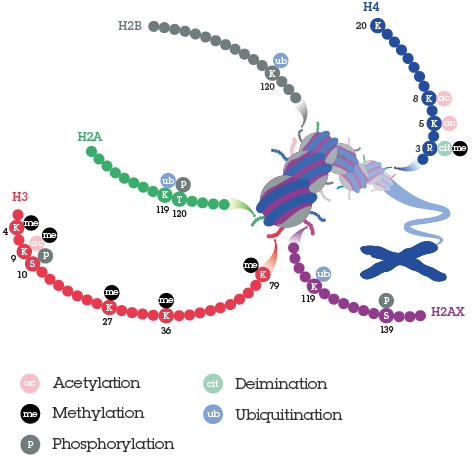
\includegraphics[width=8cm, keepaspectratio]{img/intro/hm.png}
\caption[Histon modification]{Representation of some processes involved in histone modification, influencing gene expression regulation.}
\label{fig:histmod}
\end{figure}


In particular, the \textit{Acetylation} mostly involves histones \textit{H3} and \textit{H4}, and leads to a lower grade of \gls{dna} compaction, subsequently increasing the gene expression.
\textit{Phosphorylation} highly involves positions \textit{H3S10} and \textit{T120} of \textit{H2A}, which are associated to the chromatin compaction.
It seems to be relevant for the chromosomic condensation during cellular division, for \gls{dna} damage repair and for transcription regulator.
\textit{Methylation} generally involves histones \textit{H3} and \textit{H4}, but the modification effects depend on the affected position, influencing the gene expression/repression.
More in detail, acetylation and phosphorylation directly affect the nucleosome structure, while methylation recruits multiprotein complexes involved into the chromatin remodelling.

Each of these modifications affects the \gls{dna} structure, varying not only the chromatin compaction but also by promoting, together with proteins and non-coding \gls{rna}, the chromatin folding, influencing the gene expression regulation.

%Figure \ref{fig:dnachromosome} better helps to understand the relationship between chromosomes, chromatin, nucleosomes and genes.
%
%\begin{figure}[h]
%\centering
%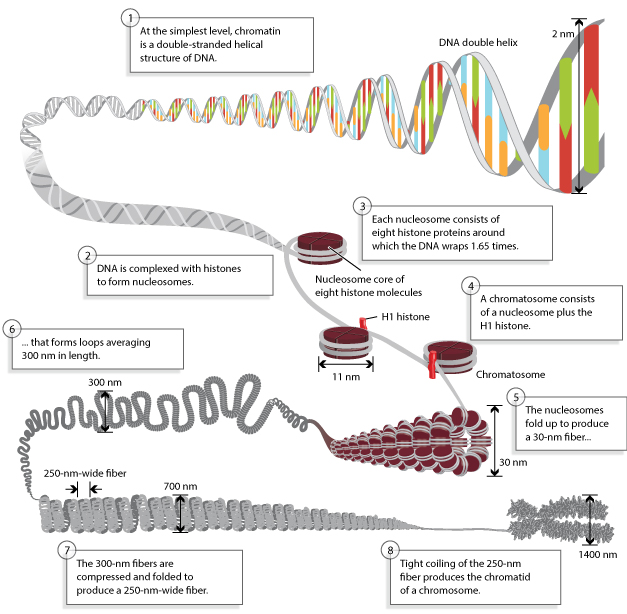
\includegraphics[width=8cm, keepaspectratio]{img/intro/dna2.jpg}
%\caption[Chromosomes and \gls{dna}]{Representation of the relation between \gls{dna} and Chromosomes.
%Inside the cell nucleus, there are pairs of chromosome, constituted by chromatin, which fundamental unit is constituted by nucleosomes, on which the \gls{dna} is wrapped around, containing the genetic information in gene form. (image adapted from \cite{Annunziato2008})}
%\label{fig:dnachromosome}
%\end{figure}

  

